\begin{figure}[!ht]
   \centering
   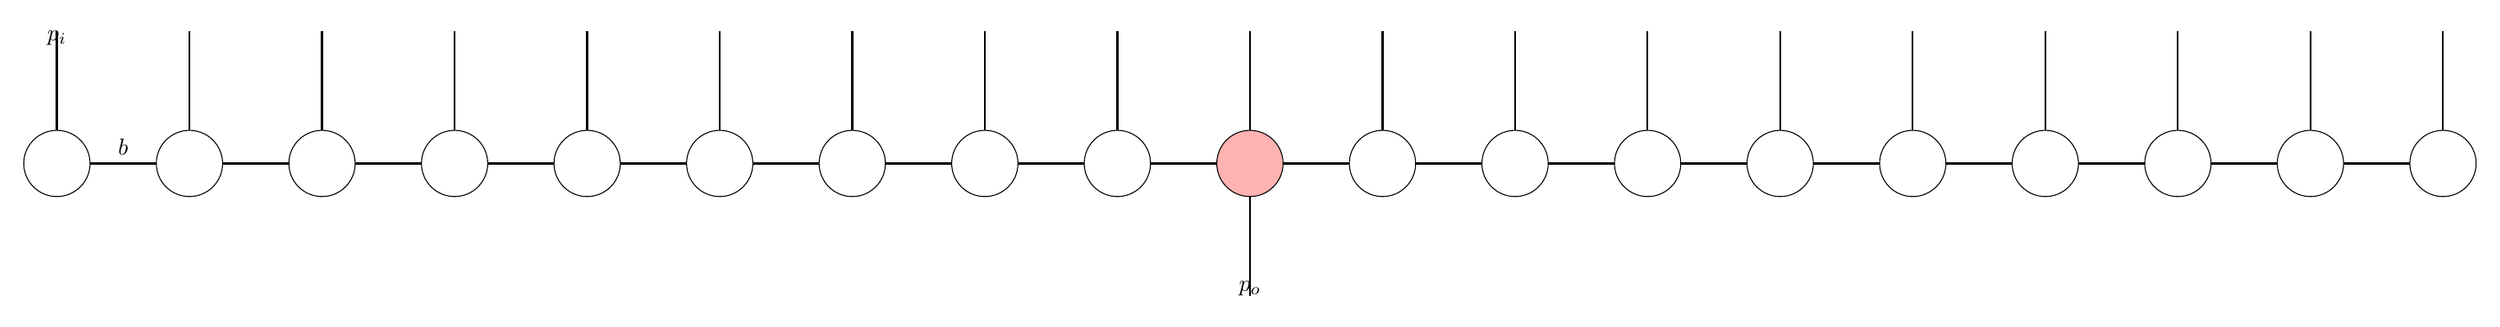
\begin{tikzpicture}[scale=2]
      %% Create a matrix site
      \tikzset
      {
      site/.style={circle, inner sep=0pt, outer sep=0pt, minimum width=1cm},
      selected site/.style = {site, fill=red!30},
      % nedge/.style = {-}
      }
      %% Sites
      \node[draw, site] (s0) at (0,0) {};
      \node[draw, site] (s1) at (1,0) {};
      \node[draw, site] (s2) at (2,0) {};
      \node[draw, site] (s3) at (3,0) {};
      \node[draw, site] (s4) at (4,0) {};
      \node[draw, site] (s5) at (5,0) {};
      \node[draw, site] (s6) at (6,0) {};
      \node[draw, site] (s7) at (7,0) {};
      \node[draw, site] (s8) at (8,0) {};
      \node[draw, selected site] (s9) at (9,0) {};
      \node[draw, site] (s10) at (10,0) {};
      \node[draw, site] (s11) at (11,0) {};
      \node[draw, site] (s12) at (12,0) {};
      \node[draw, site] (s13) at (13,0) {};
      \node[draw, site] (s14) at (14,0) {};
      \node[draw, site] (s15) at (15,0) {};
      \node[draw, site] (s16) at (16,0) {};
      \node[draw, site] (s17) at (17,0) {};
      \node[draw, site] (s18) at (18,0) {};
      %% Bonds
      \draw [thick] (s0) -- (s1) node[midway, above] {$b$} -- (s2) -- (s3) -- (s4) -- (s5) -- (s6) -- (s7) -- (s8) -- (s9) -- (s10) -- (s11) -- (s12) -- (s13) -- (s14) -- (s15) -- (s16) -- (s17) -- (s18)
      %% Incoming physical indices
      (s0) -- ++(0,1) node[midway, above=0.4cm] {$p_i$}
      (s1) -- ++(0,1)
      (s2) -- ++(0,1)
      (s3) -- ++(0,1)
      (s4) -- ++(0,1)
      (s5) -- ++(0,1)
      (s6) -- ++(0,1)
      (s7) -- ++(0,1)
      (s8) -- ++(0,1)
      (s9) -- ++(0,1)
      (s10) -- ++(0,1)
      (s11) -- ++(0,1)
      (s12) -- ++(0,1)
      (s13) -- ++(0,1)
      (s14) -- ++(0,1)
      (s15) -- ++(0,1)
      (s16) -- ++(0,1)
      (s17) -- ++(0,1)
      (s18) -- ++(0,1)
      %% Middle outline
      (s9) -- ++(0,-1) node[midway, below=0.4cm] {$p_o$};
   \end{tikzpicture}
\end{figure}